\documentclass[11pt, oneside]{report}
\usepackage{geometry}
\geometry{a4paper}
\usepackage{amsmath}
\usepackage{mathspec}  
\setmainfont [Ligatures={Common,TeX}, Numbers={OldStyle}]{Palatino Linotype} 
\setmonofont[Scale=0.85]{Menlo}
\usepackage{enumitem}
\usepackage{amssymb}
\usepackage{hyperref}
\usepackage{pgfplots}
\hypersetup{linktoc=all}

%\renewcommand{\abstractname}{Abstract}



\title{Automated Bee Pose Estimation}
\author{Jakub Nabaglo, u5558578}
\date{Semester 2, 2015}

\begin{document}
\maketitle

\begin{abstract}
    ABSTRACT
\end{abstract}

\tableofcontents\newpage

\chapter{Motivation}
    Bees play a crucial role in the environment. Acting as important pollinators for numerous flowering crops, they are relied upon by our food supply and our economy, being responsible for an estimated \$200\,billion per annum in crop production[4]. Further, bees form an integral part of our ecosystems.

    Bee populations worldwide have been decreasing for decades. Research into the causes of this decline, and ways of limiting it, is crucial. It is challenged by the difficulty in tracking bee populations. That difficulty is due to a number of factors, including a lack of trained taxonomists as well as limited resources being devoted to recording bee specimens.

    A software tool capable of automatically classifying bee species from images would hence be valuable, allowing scientists and amateurs to document bee sightings by species and thus increasing the amount of data available for research. An extension of this would be a crowdsourcing application that would enable non-professionals to photograph bees that they encouter, storing the specimen species along with a geotag and a timestamp in a public database.

\chapter{Related works}
    Santana et al. (2014) have performed automated bee classification based on bee wing images labelled with the bee species and annotated with landmarks. Their process extracts wing features such as `vein length, width, curvature, angles and the area of all cells' (Santana et al, 2014, p. 253) that may be input into a generic classifier.

    Their approach presents several problems. In order to reliably extract features, the training and testing photographs must be captured in a highly uniform manner: the wing images must be of a high resolution and have a plain white background. If the goal is to enable amateurs to photograph bees and automatically classify them, the user cannot be expected to possess the equipment or motivation necessary for such consistent specimen collection.

    Further, in the work of Santana et al. (2014), images used for training and prediction must be annotated with landmarks before relevant features can be extracted. This, again, is not something an an amateur user should be expected to do.

    As such, it is necessary to develop a method to classify bees regarding of their position or orientation in the image, without requiring the user to take the photograph in a particular way, and not necessitating that they annotate landmarks. It is a logical first step to train a machine to detect the pose of the bee, as well as the bee parts useful for classification.

    Yang and Ramanan (2011) describe a model for human pose estimation. It is a supervised learning model that trains on photographs of humans that are annotated with positions of their body parts. In addition, a tree model must be defined on these parts. The tree is used in a graphical model to take advantage of relationships between body parts during training and detection.

    Although their work describes human pose estimation, it may conceivably be applied to bee pose estimation. Challenges may include the small size of some bee parts, such as antennae or legs, as well as the tendency for bee images to occlude parts: these may lower the accuracy of part detections. Large variations in bee poses may also be problematic, as this reduces the utility of the graphical model.

\chapter{Method}
    Experiments to perform bee pose estimation were conducted on the BEES dataset. From the BEES dataset, 250 images with all seven parts labelled were selected and split into five sets of 50. Of these, four were used for training and one was used for testing. The images in BEES deemed unsuitable for use in experiments due to bee part occlusions were used as a basis for a negative training set: bees were cropped out of these images, leaving only the background.

    The algorithm described by Yang and Ramanan (2011) was used as a basis for the experiments. A tree structure was defined on the seven bee parts labelled in BEES, with the head as the root; the antennae and the thorax as children of the head; and the wings and the abdomen as children of the thorax.

    Following training on the four training sets, predictions were made on the testing set. The testing set predictions were then displayed and visually inspected for correctness and accuracy.

\section{Algorithm}
asdfasd

\section{Evaluation}
hethe

\chapter{Results}
asef

\chapter{Future direction}

asdf

\chapter{References}
%TODO use bibtex
[1] Y. Yang, D. Ramanan. Articulated Pose Estimation using Flexible Mixtures of Parts. CVPR 2011.

[2] http://www.stat.ucla.edu/~xianjie.chen/projects/pose\_estimation/pose\_estimation.html

[3] http://www.pcs.usp.br/~lti/joomla/index.php?option=com\_content\&view=article\&id=23\&Itemid=14

[4] Agriculture and Consumer Protection Department of the Food and Agriculture Organization of the United Nations


\appendix
\chapter{The BEES Dataset}
    The BEES dataset was developed for this project. It is composed of 640 photographs displaying bees of various species in diverse positions.

    Each photograph in the BEES dataset displays one bee. The bee is labelled with the coordinates in the image of the middle of its head, thorax, and abdomen, as well as the tip of its right wing, left wing, right antenna and left antenna. However, in the case that one of these bee parts is occluded, no position is listed for that part. Difficult images are also tagged, and the bee is labelled with its species.

    Figure \ref{fig:BEES_examples} shows examples of annotated images in the BEES dataset.

\begin{figure}[h]
    \centering
    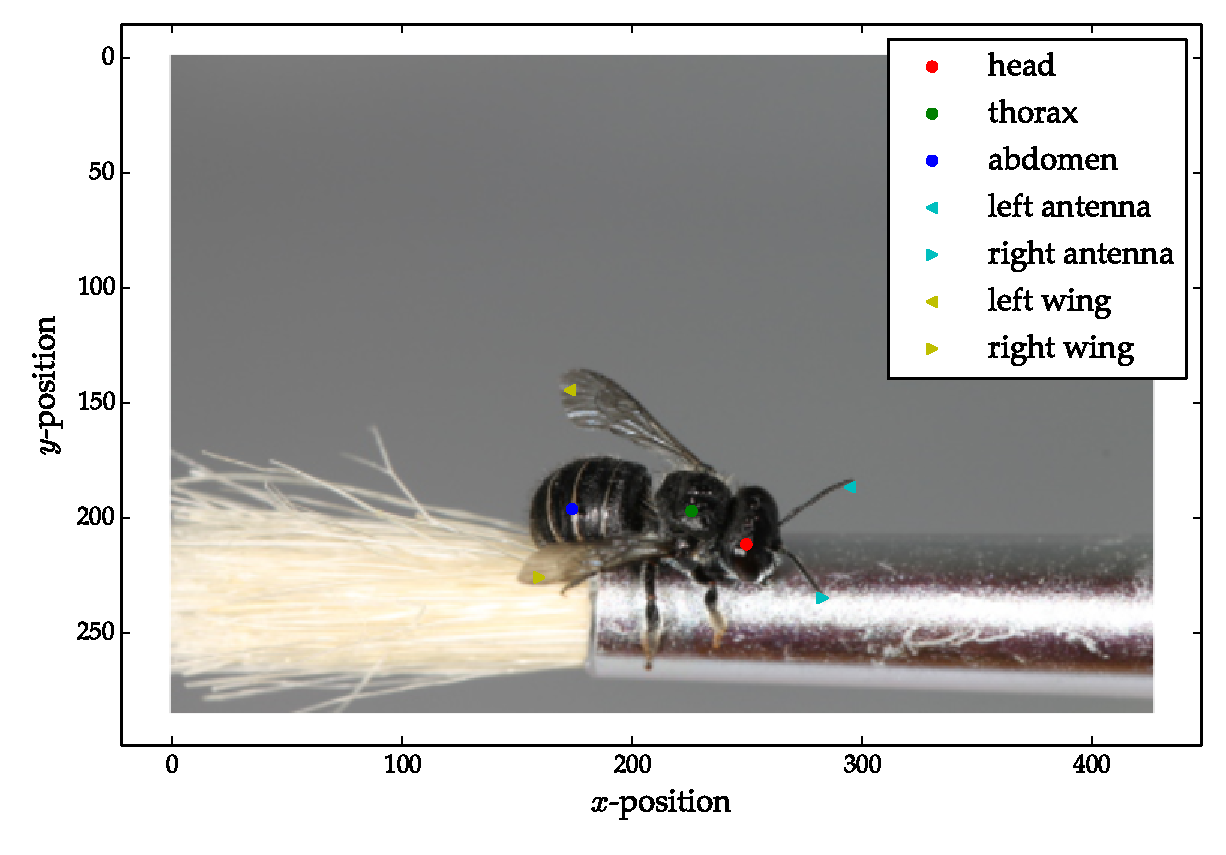
\includegraphics[width=0.45\textwidth]{b1.pdf}\quad\quad\quad
    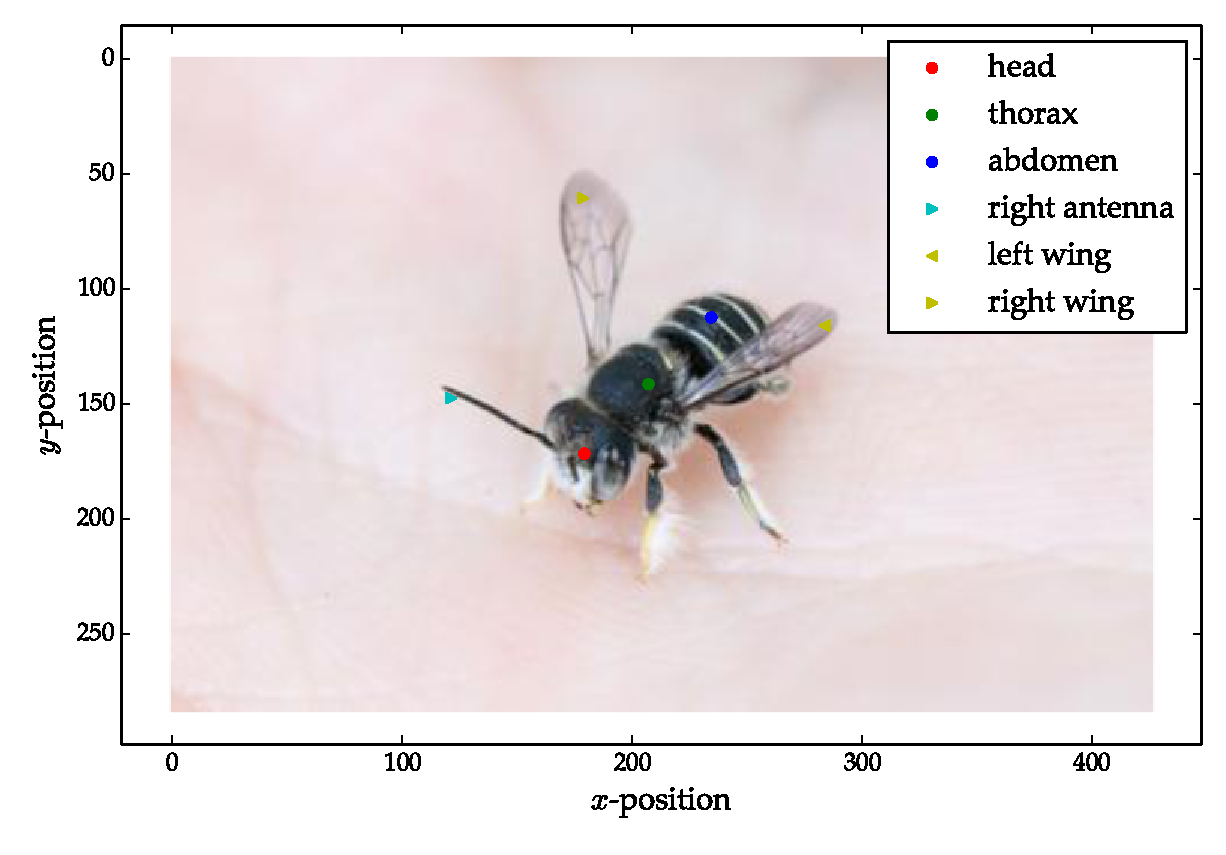
\includegraphics[width=0.45\textwidth]{b2.pdf}
    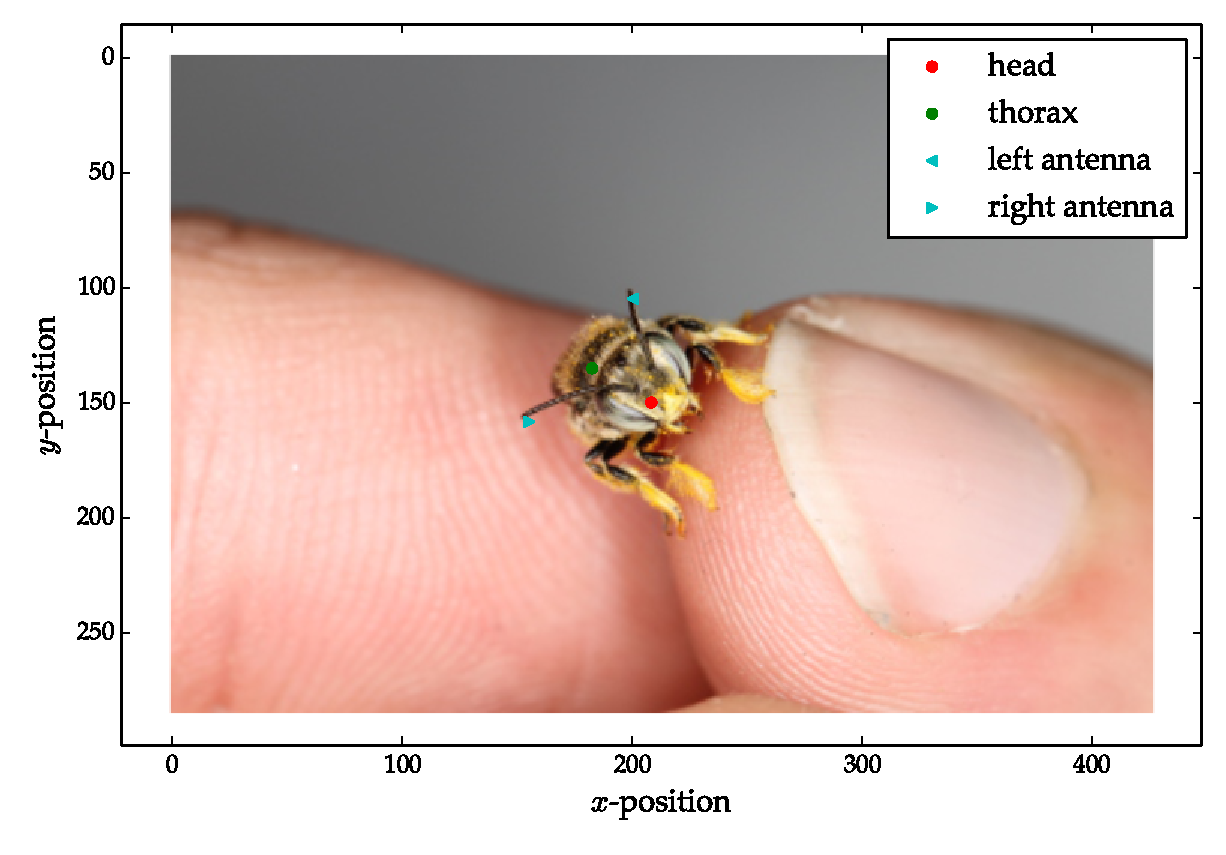
\includegraphics[width=0.45\textwidth]{b3.pdf}\quad\quad\quad
    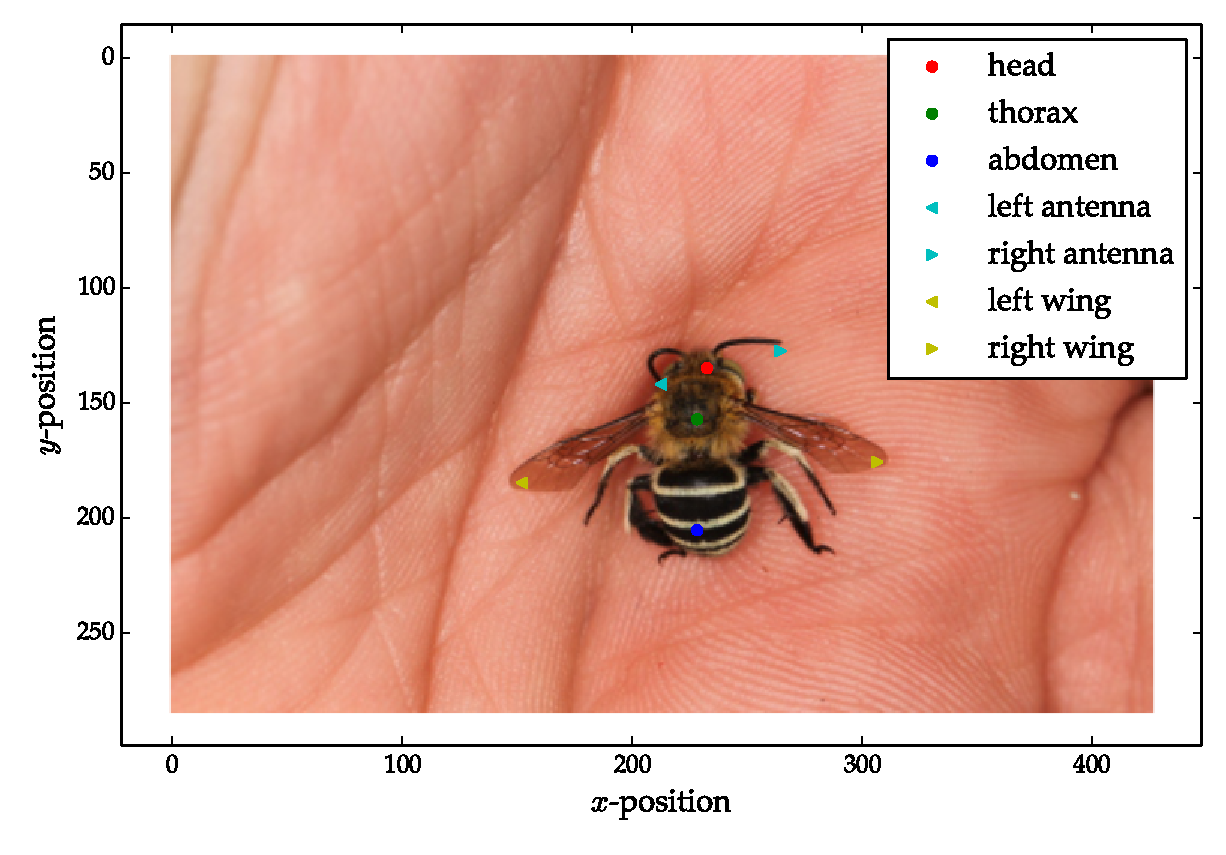
\includegraphics[width=0.45\textwidth]{b4.pdf}
    \caption{Examples of annotated images in the BEES dataset}
    \label{fig:BEES_examples}
\end{figure}

\chapter{Labelling tool}

\chapter{Python scripts}
\section{Visualisation tool}
\section{Shuffling tool}
\section{Conversion to .mat tool}
\section{Results reader}





\end{document}
